% Options for packages loaded elsewhere
\PassOptionsToPackage{unicode}{hyperref}
\PassOptionsToPackage{hyphens}{url}
%
\documentclass[
]{article}
\usepackage{amsmath,amssymb}
\usepackage{iftex}
\ifPDFTeX
  \usepackage[T1]{fontenc}
  \usepackage[utf8]{inputenc}
  \usepackage{textcomp} % provide euro and other symbols
\else % if luatex or xetex
  \usepackage{unicode-math} % this also loads fontspec
  \defaultfontfeatures{Scale=MatchLowercase}
  \defaultfontfeatures[\rmfamily]{Ligatures=TeX,Scale=1}
\fi
\usepackage{lmodern}
\ifPDFTeX\else
  % xetex/luatex font selection
\fi
% Use upquote if available, for straight quotes in verbatim environments
\IfFileExists{upquote.sty}{\usepackage{upquote}}{}
\IfFileExists{microtype.sty}{% use microtype if available
  \usepackage[]{microtype}
  \UseMicrotypeSet[protrusion]{basicmath} % disable protrusion for tt fonts
}{}
\makeatletter
\@ifundefined{KOMAClassName}{% if non-KOMA class
  \IfFileExists{parskip.sty}{%
    \usepackage{parskip}
  }{% else
    \setlength{\parindent}{0pt}
    \setlength{\parskip}{6pt plus 2pt minus 1pt}}
}{% if KOMA class
  \KOMAoptions{parskip=half}}
\makeatother
\usepackage{xcolor}
\usepackage[margin=1in]{geometry}
\usepackage{color}
\usepackage{fancyvrb}
\newcommand{\VerbBar}{|}
\newcommand{\VERB}{\Verb[commandchars=\\\{\}]}
\DefineVerbatimEnvironment{Highlighting}{Verbatim}{commandchars=\\\{\}}
% Add ',fontsize=\small' for more characters per line
\usepackage{framed}
\definecolor{shadecolor}{RGB}{248,248,248}
\newenvironment{Shaded}{\begin{snugshade}}{\end{snugshade}}
\newcommand{\AlertTok}[1]{\textcolor[rgb]{0.94,0.16,0.16}{#1}}
\newcommand{\AnnotationTok}[1]{\textcolor[rgb]{0.56,0.35,0.01}{\textbf{\textit{#1}}}}
\newcommand{\AttributeTok}[1]{\textcolor[rgb]{0.13,0.29,0.53}{#1}}
\newcommand{\BaseNTok}[1]{\textcolor[rgb]{0.00,0.00,0.81}{#1}}
\newcommand{\BuiltInTok}[1]{#1}
\newcommand{\CharTok}[1]{\textcolor[rgb]{0.31,0.60,0.02}{#1}}
\newcommand{\CommentTok}[1]{\textcolor[rgb]{0.56,0.35,0.01}{\textit{#1}}}
\newcommand{\CommentVarTok}[1]{\textcolor[rgb]{0.56,0.35,0.01}{\textbf{\textit{#1}}}}
\newcommand{\ConstantTok}[1]{\textcolor[rgb]{0.56,0.35,0.01}{#1}}
\newcommand{\ControlFlowTok}[1]{\textcolor[rgb]{0.13,0.29,0.53}{\textbf{#1}}}
\newcommand{\DataTypeTok}[1]{\textcolor[rgb]{0.13,0.29,0.53}{#1}}
\newcommand{\DecValTok}[1]{\textcolor[rgb]{0.00,0.00,0.81}{#1}}
\newcommand{\DocumentationTok}[1]{\textcolor[rgb]{0.56,0.35,0.01}{\textbf{\textit{#1}}}}
\newcommand{\ErrorTok}[1]{\textcolor[rgb]{0.64,0.00,0.00}{\textbf{#1}}}
\newcommand{\ExtensionTok}[1]{#1}
\newcommand{\FloatTok}[1]{\textcolor[rgb]{0.00,0.00,0.81}{#1}}
\newcommand{\FunctionTok}[1]{\textcolor[rgb]{0.13,0.29,0.53}{\textbf{#1}}}
\newcommand{\ImportTok}[1]{#1}
\newcommand{\InformationTok}[1]{\textcolor[rgb]{0.56,0.35,0.01}{\textbf{\textit{#1}}}}
\newcommand{\KeywordTok}[1]{\textcolor[rgb]{0.13,0.29,0.53}{\textbf{#1}}}
\newcommand{\NormalTok}[1]{#1}
\newcommand{\OperatorTok}[1]{\textcolor[rgb]{0.81,0.36,0.00}{\textbf{#1}}}
\newcommand{\OtherTok}[1]{\textcolor[rgb]{0.56,0.35,0.01}{#1}}
\newcommand{\PreprocessorTok}[1]{\textcolor[rgb]{0.56,0.35,0.01}{\textit{#1}}}
\newcommand{\RegionMarkerTok}[1]{#1}
\newcommand{\SpecialCharTok}[1]{\textcolor[rgb]{0.81,0.36,0.00}{\textbf{#1}}}
\newcommand{\SpecialStringTok}[1]{\textcolor[rgb]{0.31,0.60,0.02}{#1}}
\newcommand{\StringTok}[1]{\textcolor[rgb]{0.31,0.60,0.02}{#1}}
\newcommand{\VariableTok}[1]{\textcolor[rgb]{0.00,0.00,0.00}{#1}}
\newcommand{\VerbatimStringTok}[1]{\textcolor[rgb]{0.31,0.60,0.02}{#1}}
\newcommand{\WarningTok}[1]{\textcolor[rgb]{0.56,0.35,0.01}{\textbf{\textit{#1}}}}
\usepackage{longtable,booktabs,array}
\usepackage{calc} % for calculating minipage widths
% Correct order of tables after \paragraph or \subparagraph
\usepackage{etoolbox}
\makeatletter
\patchcmd\longtable{\par}{\if@noskipsec\mbox{}\fi\par}{}{}
\makeatother
% Allow footnotes in longtable head/foot
\IfFileExists{footnotehyper.sty}{\usepackage{footnotehyper}}{\usepackage{footnote}}
\makesavenoteenv{longtable}
\usepackage{graphicx}
\makeatletter
\def\maxwidth{\ifdim\Gin@nat@width>\linewidth\linewidth\else\Gin@nat@width\fi}
\def\maxheight{\ifdim\Gin@nat@height>\textheight\textheight\else\Gin@nat@height\fi}
\makeatother
% Scale images if necessary, so that they will not overflow the page
% margins by default, and it is still possible to overwrite the defaults
% using explicit options in \includegraphics[width, height, ...]{}
\setkeys{Gin}{width=\maxwidth,height=\maxheight,keepaspectratio}
% Set default figure placement to htbp
\makeatletter
\def\fps@figure{htbp}
\makeatother
\setlength{\emergencystretch}{3em} % prevent overfull lines
\providecommand{\tightlist}{%
  \setlength{\itemsep}{0pt}\setlength{\parskip}{0pt}}
\setcounter{secnumdepth}{-\maxdimen} % remove section numbering
\ifLuaTeX
  \usepackage{selnolig}  % disable illegal ligatures
\fi
\usepackage{bookmark}
\IfFileExists{xurl.sty}{\usepackage{xurl}}{} % add URL line breaks if available
\urlstyle{same}
\hypersetup{
  pdftitle={Data Science: Capstone (Report)},
  pdfauthor={Mael FOSSO},
  hidelinks,
  pdfcreator={LaTeX via pandoc}}

\title{Data Science: Capstone (Report)}
\author{Mael FOSSO}
\date{December 2024}

\begin{document}
\maketitle

\section{Introduction}\label{introduction}

For years, many companies have tried to build a better recommendation
algorithm from the MovieLens data set. As part of the Havard Data
Science program, we have also decided to introduce ourselves to the
recommendation algorithm world by working on MovieLens to propose a
model that will outperform the existing ones.

There are many different MovieLens data sets, each different in size: 32
MB, 1MB, 1B, 100K, 1M, 10M, 20M, 25M. In this project, we will work with
the MovieLens 10M data set. It was released in 1/2009 and consists of 10
million ratings and 100.000 tag applications applied to 100.000 movies
by 72.000 users. The MovieLens 10M data set provided for this project
was split into two.

\begin{itemize}
\tightlist
\item
  \textbf{EDX}, which contains 75\% of the dataset. It will be used to
  train a model and determine the best one.
\item
  \textbf{The Final Holdout Test}, which contains 25\% of the data set.
  It will be used for prediction purposes only.
\end{itemize}

In the real-world project, the data scientist is provided only with the
EDX data set, and the Final Holdout Test data set is nonexistent and
unknown. The Final Holdout Test is the data set used to compare each
competitor's performance in a competition. It is only kept by the
organizer and accessible to the competitors. When they submit their
model, it is evaluated with the Final Holdout Test, and the score is
displayed on the leader board. The Final Holdout Test can also be seen
as user interactions with the movie in real-time, and the model built
should predict the rating that will be given to that movie. This project
is almost similar to the 1st situation.

To obtain the best model, we will follow these steps

\begin{itemize}
\item
  Feature engineering: Create new features
\item
  Because of the large size of the EDX, instead of using
  cross-validation, we will split it into two

  \begin{itemize}
  \tightlist
  \item
    training data set to train the model
  \item
    test data set: Use to compare our different model
  \end{itemize}
\item
  Enumerate a list of algorithms or existing libraries that can be used.
  For each of them

  \begin{itemize}
  \tightlist
  \item
    Train the model with the training data set
  \item
    Use the test data set to find the best hyper-parameter
  \item
    Keep the hyper-parameter with the best RMSE
  \end{itemize}
\item
  Compare all the different models and keep the best one.
\item
  Run the best model on the Final Holdout Test and save the RMSE.
\end{itemize}

\section{Method/Analysis}\label{methodanalysis}

\subsection{Recommendation system
algorithms}\label{recommendation-system-algorithms}

In machine learning, this problem is in the class of Recommendation
Systems.

To solve a recommendation system problem, there are two approaches:

\begin{itemize}
\tightlist
\item
  Content-base filtering
\item
  Collaborative filtering
\end{itemize}

In content-based filtering, we predict the rating a user will make on a
movie based on the features of the user (age, location, etc\ldots)
and/or the feature of the movie (title, release date, genre, etc\ldots).
Either we use the features of the user to find similar users to him and
predict his rating of the movie as a function of the rating of users
similar to him, or we use the features of the movies to find similar
movies to the movie the user wants to predict and predict his rating on
that movie as a function of his rating on those similar movies.

In collaborative filtering, we predict the rating a user will give a
movie based on what similar users have given or how he is rating movies
similars to the one he wants to rate. Here, the focus is on the rating,
not on the features.

Both of them work based on the computation of similarity. The main
difference is that, in content-based filtering, the similarity between
users or movies is sought based on their characteristics, while in
collaborative filtering, the similarity is sought based on the rating
(two users are similar according to how they rate a set of movies. two
movies are similar to how a user rated them)

\subsection{Our process/approach}\label{our-processapproach}

Remember that the data was split in two:

\begin{itemize}
\tightlist
\item
  EDX for training, finding a machine learning model
\item
  Final Holdout test to determine how efficient the model
  \textbf{Question}: How to build that model
\end{itemize}

In the content-based filtering approach, we need:

\begin{itemize}
\tightlist
\item
  to know the features of the users and the movies. Unfortunately in
  this project, we don't have any user features, but we do have features
  for movies.
\item
  to build the model: there is no model but a process. A model is built
  from training and reused on a test set. In content-based filtering, we
  have a process to implement when looking for the rating of a user on a
  movie
\end{itemize}

In the collaborative filtering approach, there are two main approaches:

\begin{itemize}
\tightlist
\item
  Memory-based: It applies statistics to all data sets to make
  predictions. To find the rating \(R\) of user \(U\) to movie \(M\),

  \begin{itemize}
  \tightlist
  \item
    Find users similar to \(U\) who have rated movie \(M\)
  \item
    Calculating the rating \(R\) based on the ratings of users found in
    the previous step
  \end{itemize}
\item
  Model-based: It consists of reducing or compressing the large but
  sparse user-movie matrix through dimensionality reduction. The goal is
  to find the best \(A\) and \(B\) matrix such that they can compute
  together to have the initial user-movie matrix.
\end{itemize}

In this project, we have decided to use the \textbf{collaborative
filtering (model-based)} approach. We decided to follow that approach
because it responds to the implicit process given to us, process defined
by the two data sets provided to us: The training set and the Holdout
test set. They suggest that we should find a model from the training set
(EDX) and check how the model is good from the holdout test (The Final
Holdout test set).

The model-based approach of collaborative filtering involves finding two
matrix \(A\) and \(B\) from the user-movie matrix also called the rating
matrix \(R\) such that the product of the two matrix \(A\) and \(B\)
gives us the approximative user-movie matrix \(R\).
\[Finding A~n*k~ and B~m*k~ such that R = A x B^T\]

The real A and B do not exist. An algorithm called matrix factorization
approximates the user-movie matrix R with A and B.

The training will consist of finding the best A and B so that their
product is the closest to R based on the RMSE.

Multiple parameters intervene in the search for the best A and B. The
main one is the dimensions of A and B. Some algorithms find A and B,
such as A (nU x k) and B (k x nM). So, the training will consist of
finding the best K that reduces the RMSE. K is called the number of
factors. R = A x B. Other algorithms find A and B such that A (nU x nU)
and B (nM x nM) with a matrix in the middle of size (nU x nM) R = A x E
x B

We will implement the Matrix factorization approach, which consists of
finding the best A and B such that we have R = A x B + u + bU + bM
According to whether or not we include the bias bU and bM, we have two
models.

Also, there is the Hybrid matrix factorization, which consists of matrix
factorization based on a user's rating of a movie but also taking into
consideration the features of users and movies. It uses content-based
and collaborative data.

Taking into consideration the users/movies bias and the users/movies
features, we have

\begin{longtable}[]{@{}rcl@{}}
\toprule\noalign{}
Bias & Features & Models \\
\midrule\noalign{}
\endhead
\bottomrule\noalign{}
\endlastfoot
True & True & Model-ByFy \\
True & False & Model-ByFn \\
False & True & Model-BnFy \\
False & False & Model-BnFn \\
\end{longtable}

In R programming, there is a library called \texttt{cmfrec}, which can
handle those 4 cases. In each of them, we will only focus on finding the
excellent hyperparameter \(K\) such that \(A\) and \(B\) will be the
best in terms of smallest \texttt{RMSE}.

\subsection{Data preparation}\label{data-preparation}

We starts by preparing the data, mainly feature engineering.

\begin{itemize}
\tightlist
\item
  Extracting movie release date from movie name column
\item
  Multiple hot encoding from genre column And after that, we split the
  data to into convenient data sets to use in finding the best models
  among the 4 defined up there.
\end{itemize}

\subsubsection{Multiple-hot encoding on
Genre}\label{multiple-hot-encoding-on-genre}

The \texttt{edx} dataset contains a column named \texttt{genres}. A
movie can belong to multiple genres, and there are 18 different movie
genres. Handling string is complicated and required huge preprocessing.
One simple preprocessing data we can do, is the multiple-hot encoding.

\begin{Shaded}
\begin{Highlighting}[]
\CommentTok{\# list of all movie genres}
\NormalTok{movie\_genres }\OtherTok{\textless{}{-}} \FunctionTok{c}\NormalTok{(}\StringTok{"Action"}\NormalTok{, }\StringTok{"Adventure"}\NormalTok{, }\StringTok{"Animation"}\NormalTok{, }\StringTok{"Children"}\NormalTok{, }\StringTok{"Comedy"}\NormalTok{,}
                  \StringTok{"Crime"}\NormalTok{, }\StringTok{"Documentary"}\NormalTok{, }\StringTok{"Drama"}\NormalTok{, }\StringTok{"Fantasy"}\NormalTok{, }\StringTok{"Film{-}Noir"}\NormalTok{,}
                  \StringTok{"Horror"}\NormalTok{, }\StringTok{"Musical"}\NormalTok{, }\StringTok{"Mystery"}\NormalTok{, }\StringTok{"Romance"}\NormalTok{, }\StringTok{"Sci{-}Fi"}\NormalTok{, }\StringTok{"Thriller"}\NormalTok{,}
                  \StringTok{"War"}\NormalTok{, }\StringTok{"Western"}\NormalTok{)}

\NormalTok{genres }\OtherTok{\textless{}{-}}\NormalTok{ edx}\SpecialCharTok{$}\NormalTok{genres}

\NormalTok{split\_genre }\OtherTok{\textless{}{-}} \ControlFlowTok{function}\NormalTok{(genre) \{}
\NormalTok{  s }\OtherTok{\textless{}{-}} \FunctionTok{unlist}\NormalTok{(}\FunctionTok{str\_split}\NormalTok{(genre, }\FunctionTok{fixed}\NormalTok{(}\StringTok{"|"}\NormalTok{)))}
  
  \FunctionTok{return}\NormalTok{(}\FunctionTok{as.integer}\NormalTok{(movie\_genres }\SpecialCharTok{\%in\%}\NormalTok{ s))}
\NormalTok{\}}
\CommentTok{\# Create a data.frame with 18 columns and same number of rows than edx}
\NormalTok{genres.splitted }\OtherTok{\textless{}{-}} \FunctionTok{do.call}\NormalTok{(rbind, }\FunctionTok{lapply}\NormalTok{(genres, }\AttributeTok{FUN=}\NormalTok{split\_genre))}

\CommentTok{\# Naming the columns with the Genre name}
\FunctionTok{colnames}\NormalTok{(genres.splitted) }\OtherTok{\textless{}{-}}\NormalTok{ movie\_genres}
\end{Highlighting}
\end{Shaded}

\subsubsection{Extract year release
date}\label{extract-year-release-date}

The \texttt{edx} dataset contains a column named \texttt{title,} which
includes the movie's name and release year. We extract the release year
and use it as a movie feature like this.

\begin{Shaded}
\begin{Highlighting}[]
\FunctionTok{log\_info}\NormalTok{(}\StringTok{"Extract [year] \& [title] from movie [name]"}\NormalTok{)}

\NormalTok{movies.data }\OtherTok{\textless{}{-}}\NormalTok{ genres.splitted}
\NormalTok{movies.name.splitted }\OtherTok{\textless{}{-}}\NormalTok{ edx }\SpecialCharTok{\%\textgreater{}\%}
  \FunctionTok{mutate}\NormalTok{(}
    \AttributeTok{year =} \FunctionTok{as.integer}\NormalTok{(}\FunctionTok{str\_extract}\NormalTok{(title, }\StringTok{"(?\textless{}=}\SpecialCharTok{\textbackslash{}\textbackslash{}}\StringTok{()}\SpecialCharTok{\textbackslash{}\textbackslash{}}\StringTok{d+(?=}\SpecialCharTok{\textbackslash{}\textbackslash{}}\StringTok{)$)"}\NormalTok{)),}
    \AttributeTok{name =} \FunctionTok{str\_squish}\NormalTok{(}\FunctionTok{str\_remove}\NormalTok{(title, }\StringTok{" }\SpecialCharTok{\textbackslash{}\textbackslash{}}\StringTok{(}\SpecialCharTok{\textbackslash{}\textbackslash{}}\StringTok{d+}\SpecialCharTok{\textbackslash{}\textbackslash{}}\StringTok{)$"}\NormalTok{))}
\NormalTok{  ) }\SpecialCharTok{\%\textgreater{}\%} \FunctionTok{select}\NormalTok{(name, year)}
\NormalTok{movies.data }\OtherTok{\textless{}{-}} \FunctionTok{cbind}\NormalTok{(movies.data, }\AttributeTok{year =}\NormalTok{ movies.name.splitted}\SpecialCharTok{$}\NormalTok{year)}
\end{Highlighting}
\end{Shaded}

After creating those new features, we can create a new data frame
\texttt{edx.data} containing only features that we will use in training
the model

\begin{Shaded}
\begin{Highlighting}[]
\FunctionTok{log\_info}\NormalTok{(}\StringTok{"Create a new edx data frame with the previously created movie data"}\NormalTok{)}
\NormalTok{edx.data }\OtherTok{\textless{}{-}} \FunctionTok{cbind}\NormalTok{(edx, movies.data) }\SpecialCharTok{\%\textgreater{}\%}
  \FunctionTok{select}\NormalTok{(}\SpecialCharTok{{-}}\FunctionTok{c}\NormalTok{(title, genres))}
\end{Highlighting}
\end{Shaded}

\subsubsection{Build the training and validation
dataset}\label{build-the-training-and-validation-dataset}

As we have to find the best K, the process consists of splitting the
training data set \texttt{edx.data} into training and validation data
sets. The training data set will be used to create the model, and the
validation dataset will be used to evaluate the obtained model. The
process is always used for finding the best hyperparameters.

We will split our \texttt{edx.data} data set into 80\% for training and
20\% for validation.

\begin{Shaded}
\begin{Highlighting}[]
\FunctionTok{set.seed}\NormalTok{(}\DecValTok{1}\NormalTok{, }\AttributeTok{sample.kind=}\StringTok{"Rounding"}\NormalTok{) }\CommentTok{\# if using R 3.6 or later}
\CommentTok{\# set.seed(1) \# if using R 3.5 or earlier}
\NormalTok{validation\_index }\OtherTok{\textless{}{-}} \FunctionTok{createDataPartition}\NormalTok{(}\AttributeTok{y =}\NormalTok{ edx.data}\SpecialCharTok{$}\NormalTok{rating, }\AttributeTok{times =} \DecValTok{1}\NormalTok{, }\AttributeTok{p =} \FloatTok{0.25}\NormalTok{, }\AttributeTok{list =} \ConstantTok{FALSE}\NormalTok{)}
\NormalTok{train.edx }\OtherTok{\textless{}{-}}\NormalTok{ edx.data[}\SpecialCharTok{{-}}\NormalTok{validation\_index,]}
\NormalTok{temp }\OtherTok{\textless{}{-}}\NormalTok{ edx.data[validation\_index,]}

\CommentTok{\# Make sure userId and movieId in final hold{-}out validation set are also in edx set}
\NormalTok{validation.edx }\OtherTok{\textless{}{-}}\NormalTok{ temp }\SpecialCharTok{\%\textgreater{}\%}
  \FunctionTok{semi\_join}\NormalTok{(train.edx, }\AttributeTok{by =} \StringTok{"movieId"}\NormalTok{) }\SpecialCharTok{\%\textgreater{}\%}
  \FunctionTok{semi\_join}\NormalTok{(train.edx, }\AttributeTok{by =} \StringTok{"userId"}\NormalTok{)}

\CommentTok{\# Add rows removed from final hold{-}out validation set back into edx set}
\NormalTok{removed }\OtherTok{\textless{}{-}} \FunctionTok{anti\_join}\NormalTok{(temp, validation.edx)}
\NormalTok{train.edx }\OtherTok{\textless{}{-}} \FunctionTok{rbind}\NormalTok{(train.edx, removed)}

\FunctionTok{rm}\NormalTok{(validation\_index, temp, removed)}
\end{Highlighting}
\end{Shaded}

Once splitting the \texttt{edx} dataset, we then prepare the different
data frame, so that they can be used in training and validation

\begin{Shaded}
\begin{Highlighting}[]
\DocumentationTok{\#\# Extract (userId, movieId, rating) data frame from EDX}
\NormalTok{X }\OtherTok{\textless{}{-}}\NormalTok{ edx.data }\SpecialCharTok{\%\textgreater{}\%} \FunctionTok{select}\NormalTok{(userId, movieId, rating) }\CommentTok{\# will be use to train the best model with all the training \textasciigrave{}edx\textasciigrave{} data.}

\DocumentationTok{\#\# Extract (userId, movieId, rating) data frame from the Final hold{-}out test}
\NormalTok{X.fht }\OtherTok{\textless{}{-}}\NormalTok{ final\_holdout\_test }\SpecialCharTok{\%\textgreater{}\%} \FunctionTok{select}\NormalTok{(userId, movieId, rating)}

\DocumentationTok{\#\# Extract (userId, movieId, rating) data frame for training and validation}
\NormalTok{X.train }\OtherTok{\textless{}{-}}\NormalTok{ train.edx }\SpecialCharTok{\%\textgreater{}\%} \FunctionTok{select}\NormalTok{(userId, movieId, rating)}
\NormalTok{X.validation }\OtherTok{\textless{}{-}}\NormalTok{ validation.edx }\SpecialCharTok{\%\textgreater{}\%} \FunctionTok{select}\NormalTok{(userId, movieId, rating)}

\DocumentationTok{\#\# Build data frame containing only movie features}
\NormalTok{X.train.movies }\OtherTok{\textless{}{-}}\NormalTok{ train.edx }\SpecialCharTok{\%\textgreater{}\%} \FunctionTok{select}\NormalTok{(}\SpecialCharTok{{-}}\FunctionTok{c}\NormalTok{(userId, movieId, rating))}
\NormalTok{X.train.movies }\OtherTok{\textless{}{-}} \FunctionTok{scale}\NormalTok{(X.train.movies)}

\NormalTok{X.validation.movies }\OtherTok{\textless{}{-}}\NormalTok{ validation.edx }\SpecialCharTok{\%\textgreater{}\%} \FunctionTok{select}\NormalTok{(}\SpecialCharTok{{-}}\FunctionTok{c}\NormalTok{(userId, movieId, rating))}
\NormalTok{X.validation.movies }\OtherTok{\textless{}{-}} \FunctionTok{scale}\NormalTok{(X.validation.movies)}

\NormalTok{X.movies }\OtherTok{\textless{}{-}}\NormalTok{ edx.data }\SpecialCharTok{\%\textgreater{}\%} \FunctionTok{select}\NormalTok{(}\SpecialCharTok{{-}}\FunctionTok{c}\NormalTok{(userId, movieId, }\SpecialCharTok{**}\NormalTok{rating}\SpecialCharTok{**}\NormalTok{)) }\CommentTok{\# Movie data from multiple hot encoding}
\end{Highlighting}
\end{Shaded}

We can now, after those step, start finding the best models.

\subsection{Finding the best models.}\label{finding-the-best-models.}

Remember that we said that there was 4 models.

\begin{longtable}[]{@{}rcl@{}}
\toprule\noalign{}
Bias & Features & Models \\
\midrule\noalign{}
\endhead
\bottomrule\noalign{}
\endlastfoot
True & True & Model-ByFy \\
True & False & Model-ByFn \\
False & True & Model-BnFy \\
False & False & Model-BnFn \\
\end{longtable}

Finding the best models consist of

\begin{enumerate}
\def\labelenumi{\arabic{enumi}.}
\tightlist
\item
  finding the best K for each of the 4 models
\item
  then finding the best models between those 4 selected one previously.
\end{enumerate}

For each of our models, we ran the \texttt{CMF} algorithm, with good
parameters for each value of K from 3 to 30. For each K, we train the
model using \texttt{X.train} and \texttt{X.train.movies} if needed to
obtain a model and then compute the validation error from
\texttt{X.validation}.

\subsubsection{Model-ByFy: With bias and movies
features}\label{model-byfy-with-bias-and-movies-features}

\begin{Shaded}
\begin{Highlighting}[]
\NormalTok{errors }\OtherTok{\textless{}{-}} \FunctionTok{c}\NormalTok{()}
\NormalTok{best\_model }\OtherTok{\textless{}{-}} \ConstantTok{NULL}
\NormalTok{best\_error }\OtherTok{\textless{}{-}} \FloatTok{10e6}

\NormalTok{startTime }\OtherTok{\textless{}{-}} \FunctionTok{Sys.time}\NormalTok{()}
\ControlFlowTok{for}\NormalTok{ (k }\ControlFlowTok{in} \DecValTok{3}\SpecialCharTok{:}\DecValTok{30}\NormalTok{) \{}
 \FunctionTok{log\_info}\NormalTok{(}\StringTok{"Start k=\{k\}"}\NormalTok{)}
\NormalTok{ model }\OtherTok{\textless{}{-}} \FunctionTok{CMF}\NormalTok{(X.train, }\AttributeTok{I =}\NormalTok{ X.train.movies, }\AttributeTok{k =}\NormalTok{ k, }\AttributeTok{method =} \StringTok{\textquotesingle{}lbfgs\textquotesingle{}}\NormalTok{,}
              \AttributeTok{user\_bias =} \ConstantTok{TRUE}\NormalTok{, }\AttributeTok{item\_bias =} \ConstantTok{TRUE}\NormalTok{,}
              \AttributeTok{center =} \ConstantTok{TRUE}\NormalTok{,}
              \CommentTok{\# NA\_as\_zero = TRUE,}
              \AttributeTok{nthreads =} \DecValTok{1}\NormalTok{, }\AttributeTok{verbose =} \ConstantTok{FALSE}\NormalTok{, }\AttributeTok{seed =} \DecValTok{1}\NormalTok{)}

\NormalTok{ predictions }\OtherTok{\textless{}{-}} \FunctionTok{predict}\NormalTok{(model, }\AttributeTok{user=}\NormalTok{X.validation}\SpecialCharTok{$}\NormalTok{userId, }\AttributeTok{item=}\NormalTok{X.validation}\SpecialCharTok{$}\NormalTok{movieId)}
\NormalTok{ k\_errors }\OtherTok{\textless{}{-}} \FunctionTok{RMSE}\NormalTok{(X.validation}\SpecialCharTok{$}\NormalTok{rating, predictions)}

 \ControlFlowTok{if}\NormalTok{ (k\_errors }\SpecialCharTok{\textless{}}\NormalTok{ best\_error) \{}
\NormalTok{   best\_model }\OtherTok{\textless{}{-}}\NormalTok{ model}
\NormalTok{   best\_error }\OtherTok{\textless{}{-}}\NormalTok{ k\_errors}
\NormalTok{ \}}

\NormalTok{ errors }\OtherTok{\textless{}{-}} \FunctionTok{c}\NormalTok{(errors, k\_errors)}
 \FunctionTok{log\_info}\NormalTok{(}\StringTok{"End k=\{k\}; Error=\{k\_errors\}"}\NormalTok{)}
\NormalTok{\}}
\end{Highlighting}
\end{Shaded}

\subsubsection{Model-ByFn: With bias but without movies
features}\label{model-byfn-with-bias-but-without-movies-features}

\begin{Shaded}
\begin{Highlighting}[]
\NormalTok{errors }\OtherTok{\textless{}{-}} \FunctionTok{c}\NormalTok{()}
\NormalTok{best\_model }\OtherTok{\textless{}{-}} \ConstantTok{NULL}
\NormalTok{best\_error }\OtherTok{\textless{}{-}} \FloatTok{10e6}

\NormalTok{startTime }\OtherTok{\textless{}{-}} \FunctionTok{Sys.time}\NormalTok{()}
\ControlFlowTok{for}\NormalTok{ (k }\ControlFlowTok{in} \DecValTok{3}\SpecialCharTok{:}\DecValTok{30}\NormalTok{) \{}
  \FunctionTok{log\_info}\NormalTok{(}\StringTok{"Start k=\{k\}"}\NormalTok{)}
\NormalTok{  model }\OtherTok{\textless{}{-}} \FunctionTok{CMF}\NormalTok{(X.train, }\AttributeTok{k =}\NormalTok{ k, }\AttributeTok{method =} \StringTok{\textquotesingle{}lbfgs\textquotesingle{}}\NormalTok{,}
               \AttributeTok{user\_bias =} \ConstantTok{TRUE}\NormalTok{, }\AttributeTok{item\_bias =} \ConstantTok{TRUE}\NormalTok{,}
              \AttributeTok{center =} \ConstantTok{TRUE}\NormalTok{,}
              \CommentTok{\# NA\_as\_zero = TRUE, }
              \AttributeTok{nthreads =} \DecValTok{1}\NormalTok{, }\AttributeTok{verbose =} \ConstantTok{FALSE}\NormalTok{, }\AttributeTok{seed =} \DecValTok{1}\NormalTok{)}
 
\NormalTok{ predictions }\OtherTok{\textless{}{-}} \FunctionTok{predict}\NormalTok{(model, }\AttributeTok{user=}\NormalTok{X.validation}\SpecialCharTok{$}\NormalTok{userId, }\AttributeTok{item=}\NormalTok{X.validation}\SpecialCharTok{$}\NormalTok{movieId)}
\NormalTok{ k\_errors }\OtherTok{\textless{}{-}} \FunctionTok{RMSE}\NormalTok{(X.validation}\SpecialCharTok{$}\NormalTok{rating, predictions)}
 
 \ControlFlowTok{if}\NormalTok{ (k\_errors }\SpecialCharTok{\textless{}}\NormalTok{ best\_error) \{}
\NormalTok{   best\_model }\OtherTok{\textless{}{-}}\NormalTok{ model}
\NormalTok{   best\_error }\OtherTok{\textless{}{-}}\NormalTok{ k\_errors}
\NormalTok{ \}}
  
\NormalTok{ errors }\OtherTok{\textless{}{-}} \FunctionTok{c}\NormalTok{(errors, k\_errors)}
 \FunctionTok{log\_info}\NormalTok{(}\StringTok{"End k=\{k\}; Error=\{k\_errors\}"}\NormalTok{)}
\NormalTok{\}}
\NormalTok{endTime }\OtherTok{\textless{}{-}} \FunctionTok{Sys.time}\NormalTok{()}
\end{Highlighting}
\end{Shaded}

\subsubsection{Model-BnFy: Without bias but with movies
features}\label{model-bnfy-without-bias-but-with-movies-features}

\begin{Shaded}
\begin{Highlighting}[]
\NormalTok{errors }\OtherTok{\textless{}{-}} \FunctionTok{c}\NormalTok{()}
\NormalTok{best\_model }\OtherTok{\textless{}{-}} \ConstantTok{NULL}
\NormalTok{best\_error }\OtherTok{\textless{}{-}} \FloatTok{10e6}

\NormalTok{startTime }\OtherTok{\textless{}{-}} \FunctionTok{Sys.time}\NormalTok{()}
\ControlFlowTok{for}\NormalTok{ (k }\ControlFlowTok{in} \DecValTok{3}\SpecialCharTok{:}\DecValTok{30}\NormalTok{) \{}
  \FunctionTok{log\_info}\NormalTok{(}\StringTok{"Start k=\{k\}"}\NormalTok{)}
\NormalTok{  model }\OtherTok{\textless{}{-}} \FunctionTok{CMF}\NormalTok{(X.train, }\AttributeTok{k =}\NormalTok{ k, }\AttributeTok{method =} \StringTok{\textquotesingle{}lbfgs\textquotesingle{}}\NormalTok{,}
               \AttributeTok{user\_bias =} \ConstantTok{FALSE}\NormalTok{, }\AttributeTok{item\_bias =} \ConstantTok{FALSE}\NormalTok{,}
               \AttributeTok{center =} \ConstantTok{TRUE}\NormalTok{,}
               \CommentTok{\# NA\_as\_zero = TRUE,}
               \AttributeTok{nthreads =} \DecValTok{1}\NormalTok{, }\AttributeTok{verbose =} \ConstantTok{FALSE}\NormalTok{, }\AttributeTok{seed =} \DecValTok{1}\NormalTok{)}

\NormalTok{  predictions }\OtherTok{\textless{}{-}} \FunctionTok{predict}\NormalTok{(model, }\AttributeTok{user=}\NormalTok{X.validation}\SpecialCharTok{$}\NormalTok{userId, }\AttributeTok{item=}\NormalTok{X.validation}\SpecialCharTok{$}\NormalTok{movieId)}
\NormalTok{  k\_errors }\OtherTok{\textless{}{-}} \FunctionTok{RMSE}\NormalTok{(X.validation}\SpecialCharTok{$}\NormalTok{rating, predictions)}

  \ControlFlowTok{if}\NormalTok{ (k\_errors }\SpecialCharTok{\textless{}}\NormalTok{ best\_error) \{}
\NormalTok{    best\_model }\OtherTok{\textless{}{-}}\NormalTok{ model}
\NormalTok{    best\_error }\OtherTok{\textless{}{-}}\NormalTok{ k\_errors}
\NormalTok{  \}}

\NormalTok{  errors }\OtherTok{\textless{}{-}} \FunctionTok{c}\NormalTok{(errors, k\_errors)}
  \FunctionTok{log\_info}\NormalTok{(}\StringTok{"End k=\{k\}; Error=\{k\_errors\}"}\NormalTok{)}
\NormalTok{\}}
\NormalTok{endTime }\OtherTok{\textless{}{-}} \FunctionTok{Sys.time}\NormalTok{()}
\end{Highlighting}
\end{Shaded}

\subsubsection{Model-BnFn: Without bias and movies
features}\label{model-bnfn-without-bias-and-movies-features}

\begin{Shaded}
\begin{Highlighting}[]
\NormalTok{errors }\OtherTok{\textless{}{-}} \FunctionTok{c}\NormalTok{()}
\NormalTok{best\_model }\OtherTok{\textless{}{-}} \ConstantTok{NULL}
\NormalTok{best\_error }\OtherTok{\textless{}{-}} \FloatTok{10e6}

\NormalTok{startTime }\OtherTok{\textless{}{-}} \FunctionTok{Sys.time}\NormalTok{()}
\ControlFlowTok{for}\NormalTok{ (k }\ControlFlowTok{in} \DecValTok{3}\SpecialCharTok{:}\DecValTok{30}\NormalTok{) \{}
 \FunctionTok{log\_info}\NormalTok{(}\StringTok{"Start k=\{k\}"}\NormalTok{)}
\NormalTok{ model }\OtherTok{\textless{}{-}} \FunctionTok{CMF}\NormalTok{(X.train, }\AttributeTok{k =}\NormalTok{ k, }\AttributeTok{method =} \StringTok{\textquotesingle{}lbfgs\textquotesingle{}}\NormalTok{,}
              \AttributeTok{user\_bias =} \ConstantTok{FALSE}\NormalTok{, }\AttributeTok{item\_bias =} \ConstantTok{FALSE}\NormalTok{,}
              \AttributeTok{center =} \ConstantTok{TRUE}\NormalTok{,}
              \CommentTok{\# NA\_as\_zero = TRUE, }
              \AttributeTok{nthreads =} \DecValTok{1}\NormalTok{, }\AttributeTok{verbose =} \ConstantTok{FALSE}\NormalTok{, }\AttributeTok{seed =} \DecValTok{1}\NormalTok{)}
  
\NormalTok{ predictions }\OtherTok{\textless{}{-}} \FunctionTok{predict}\NormalTok{(model, }\AttributeTok{user=}\NormalTok{X.validation}\SpecialCharTok{$}\NormalTok{userId, }\AttributeTok{item=}\NormalTok{X.validation}\SpecialCharTok{$}\NormalTok{movieId)}
\NormalTok{ k\_errors }\OtherTok{\textless{}{-}} \FunctionTok{RMSE}\NormalTok{(X.validation}\SpecialCharTok{$}\NormalTok{rating, predictions)}
  
 \ControlFlowTok{if}\NormalTok{ (k\_errors }\SpecialCharTok{\textless{}}\NormalTok{ best\_error) \{}
\NormalTok{   best\_model }\OtherTok{\textless{}{-}}\NormalTok{ model}
\NormalTok{   best\_error }\OtherTok{\textless{}{-}}\NormalTok{ k\_errors}
\NormalTok{ \}}
  
\NormalTok{ errors }\OtherTok{\textless{}{-}} \FunctionTok{c}\NormalTok{(errors, k\_errors)}
 \FunctionTok{log\_info}\NormalTok{(}\StringTok{"End k=\{k\}; Error=\{k\_errors\}"}\NormalTok{)}
\NormalTok{\}}
\NormalTok{endTime }\OtherTok{\textless{}{-}} \FunctionTok{Sys.time}\NormalTok{()}
\end{Highlighting}
\end{Shaded}

\section{Results}\label{results}

At the end of the execution of each of those 4 models, we ploted a chart
of the \texttt{RMSE} function to \texttt{K}. Here is the 4 chart.

\begin{figure}
\centering
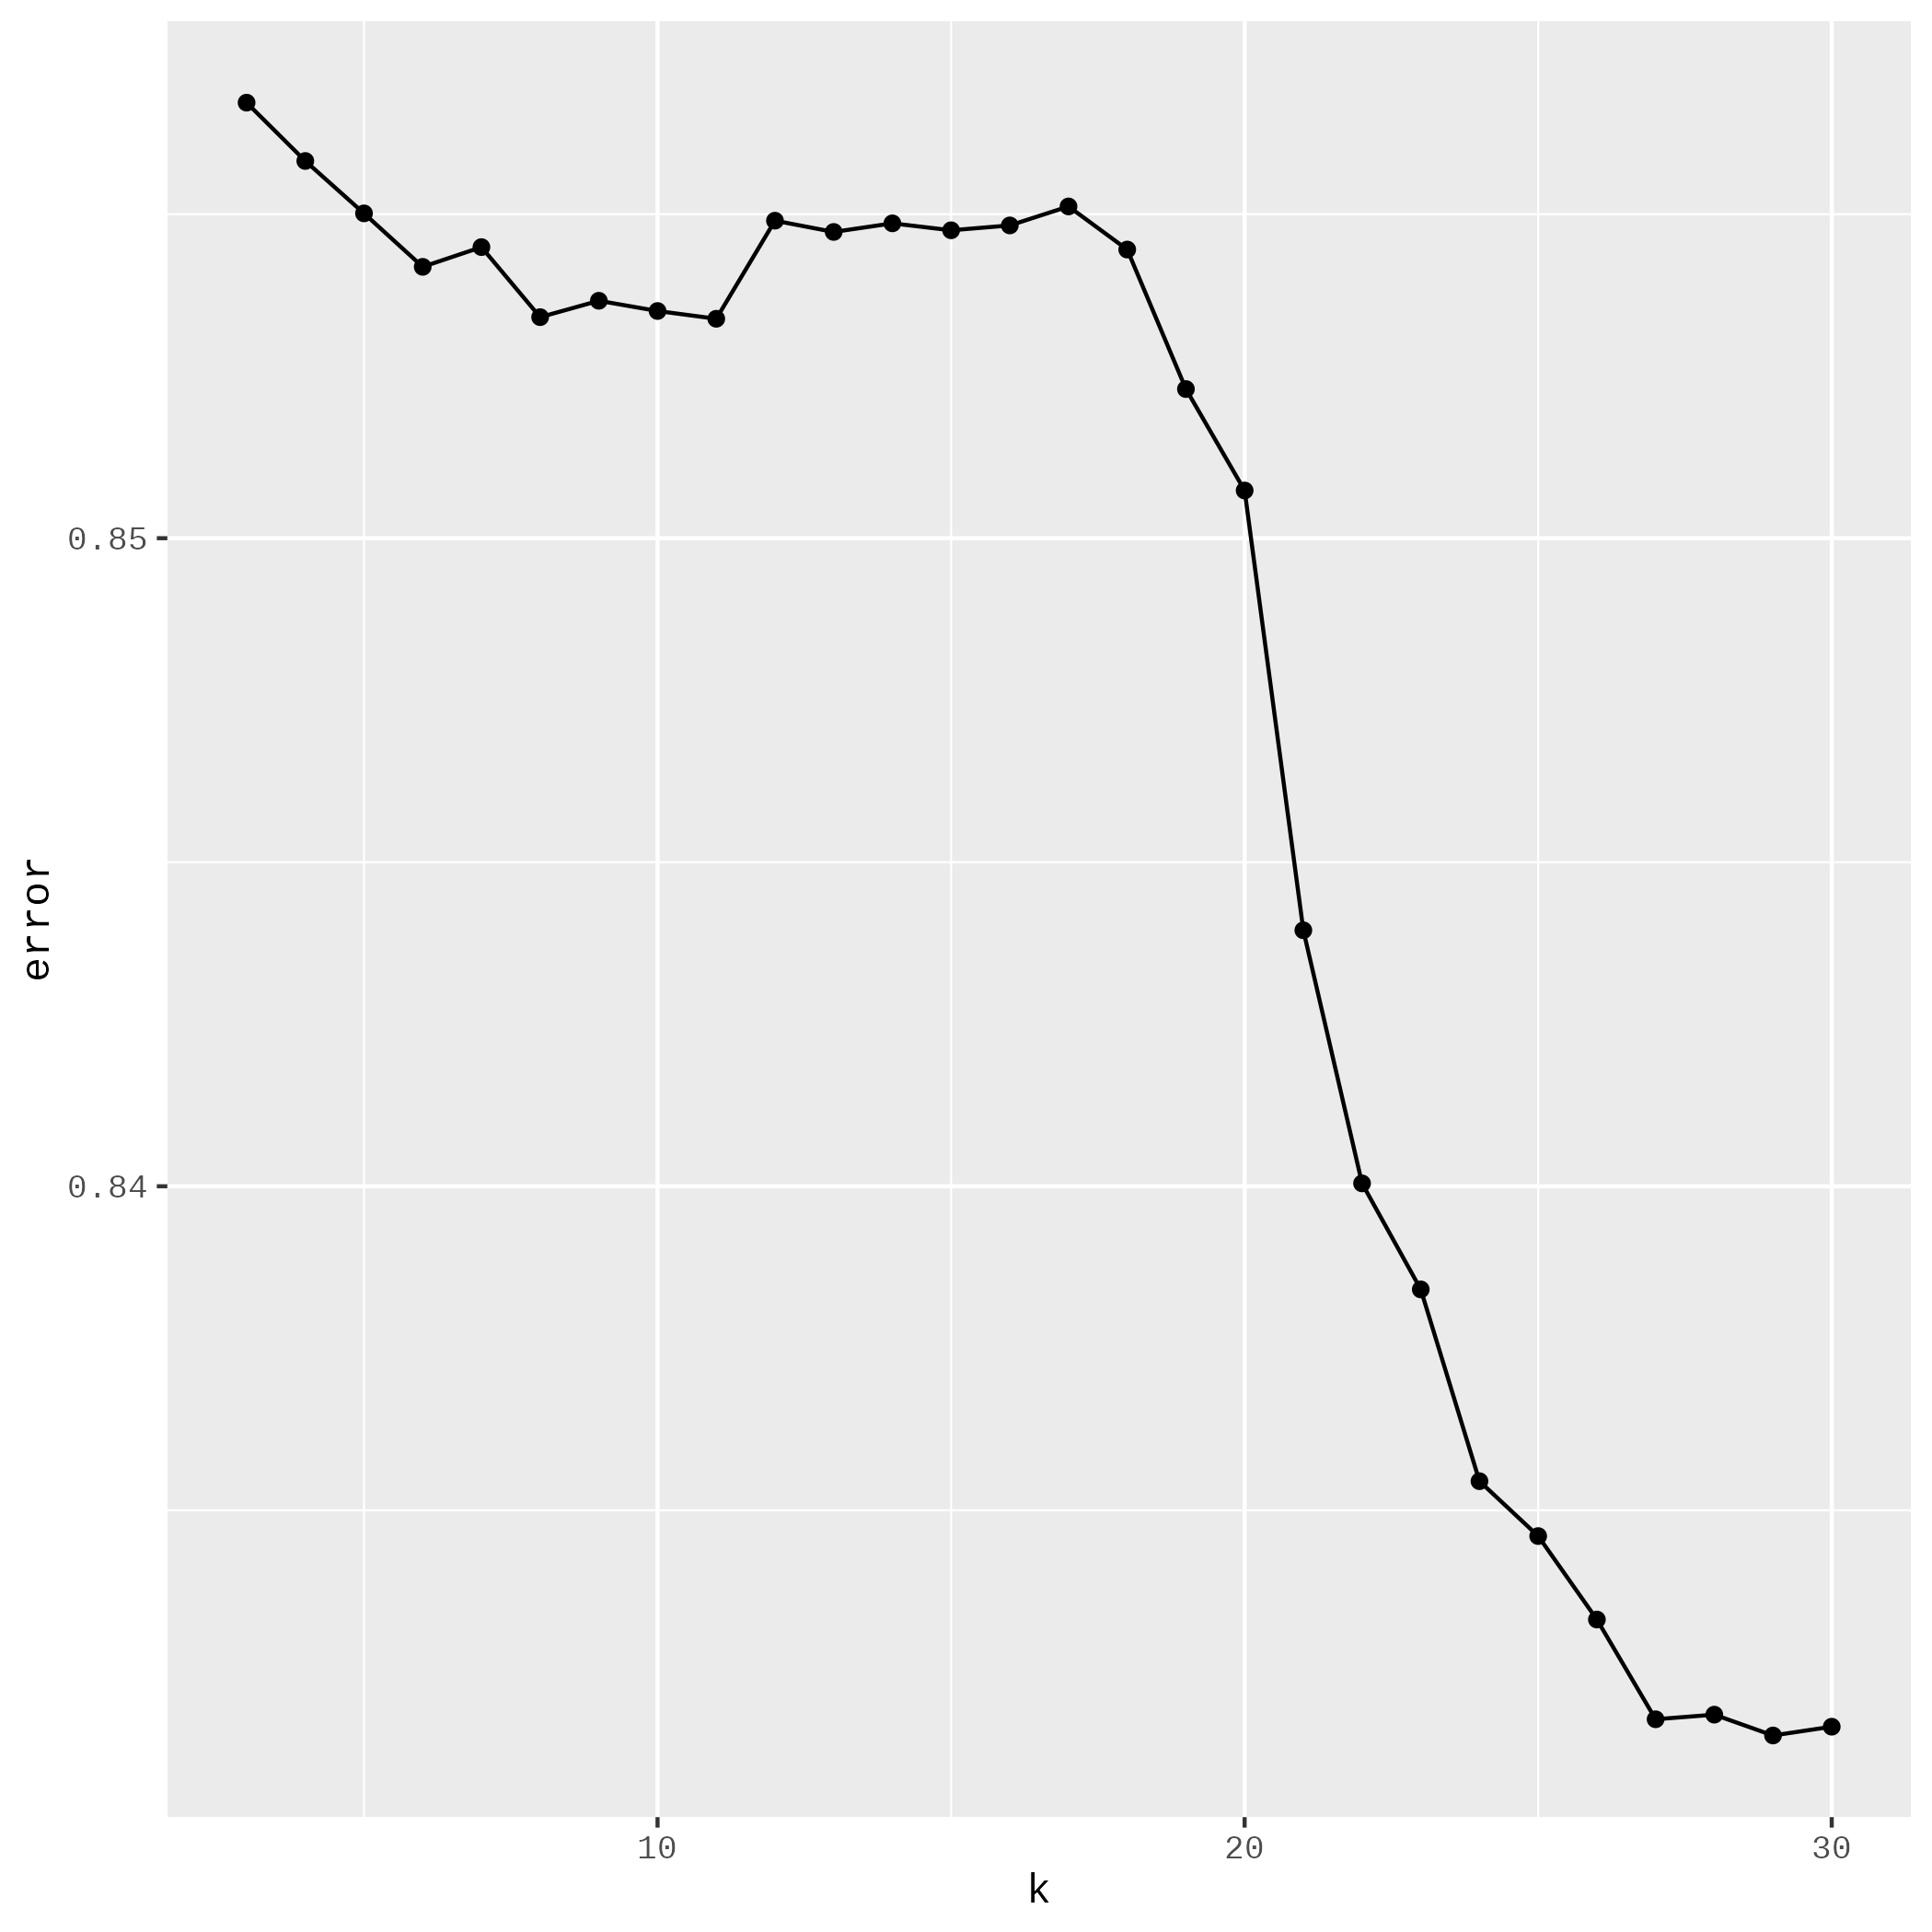
\includegraphics{./model-bias-movies.png}
\caption{With bias and movies data}
\end{figure}

\begin{figure}
\centering
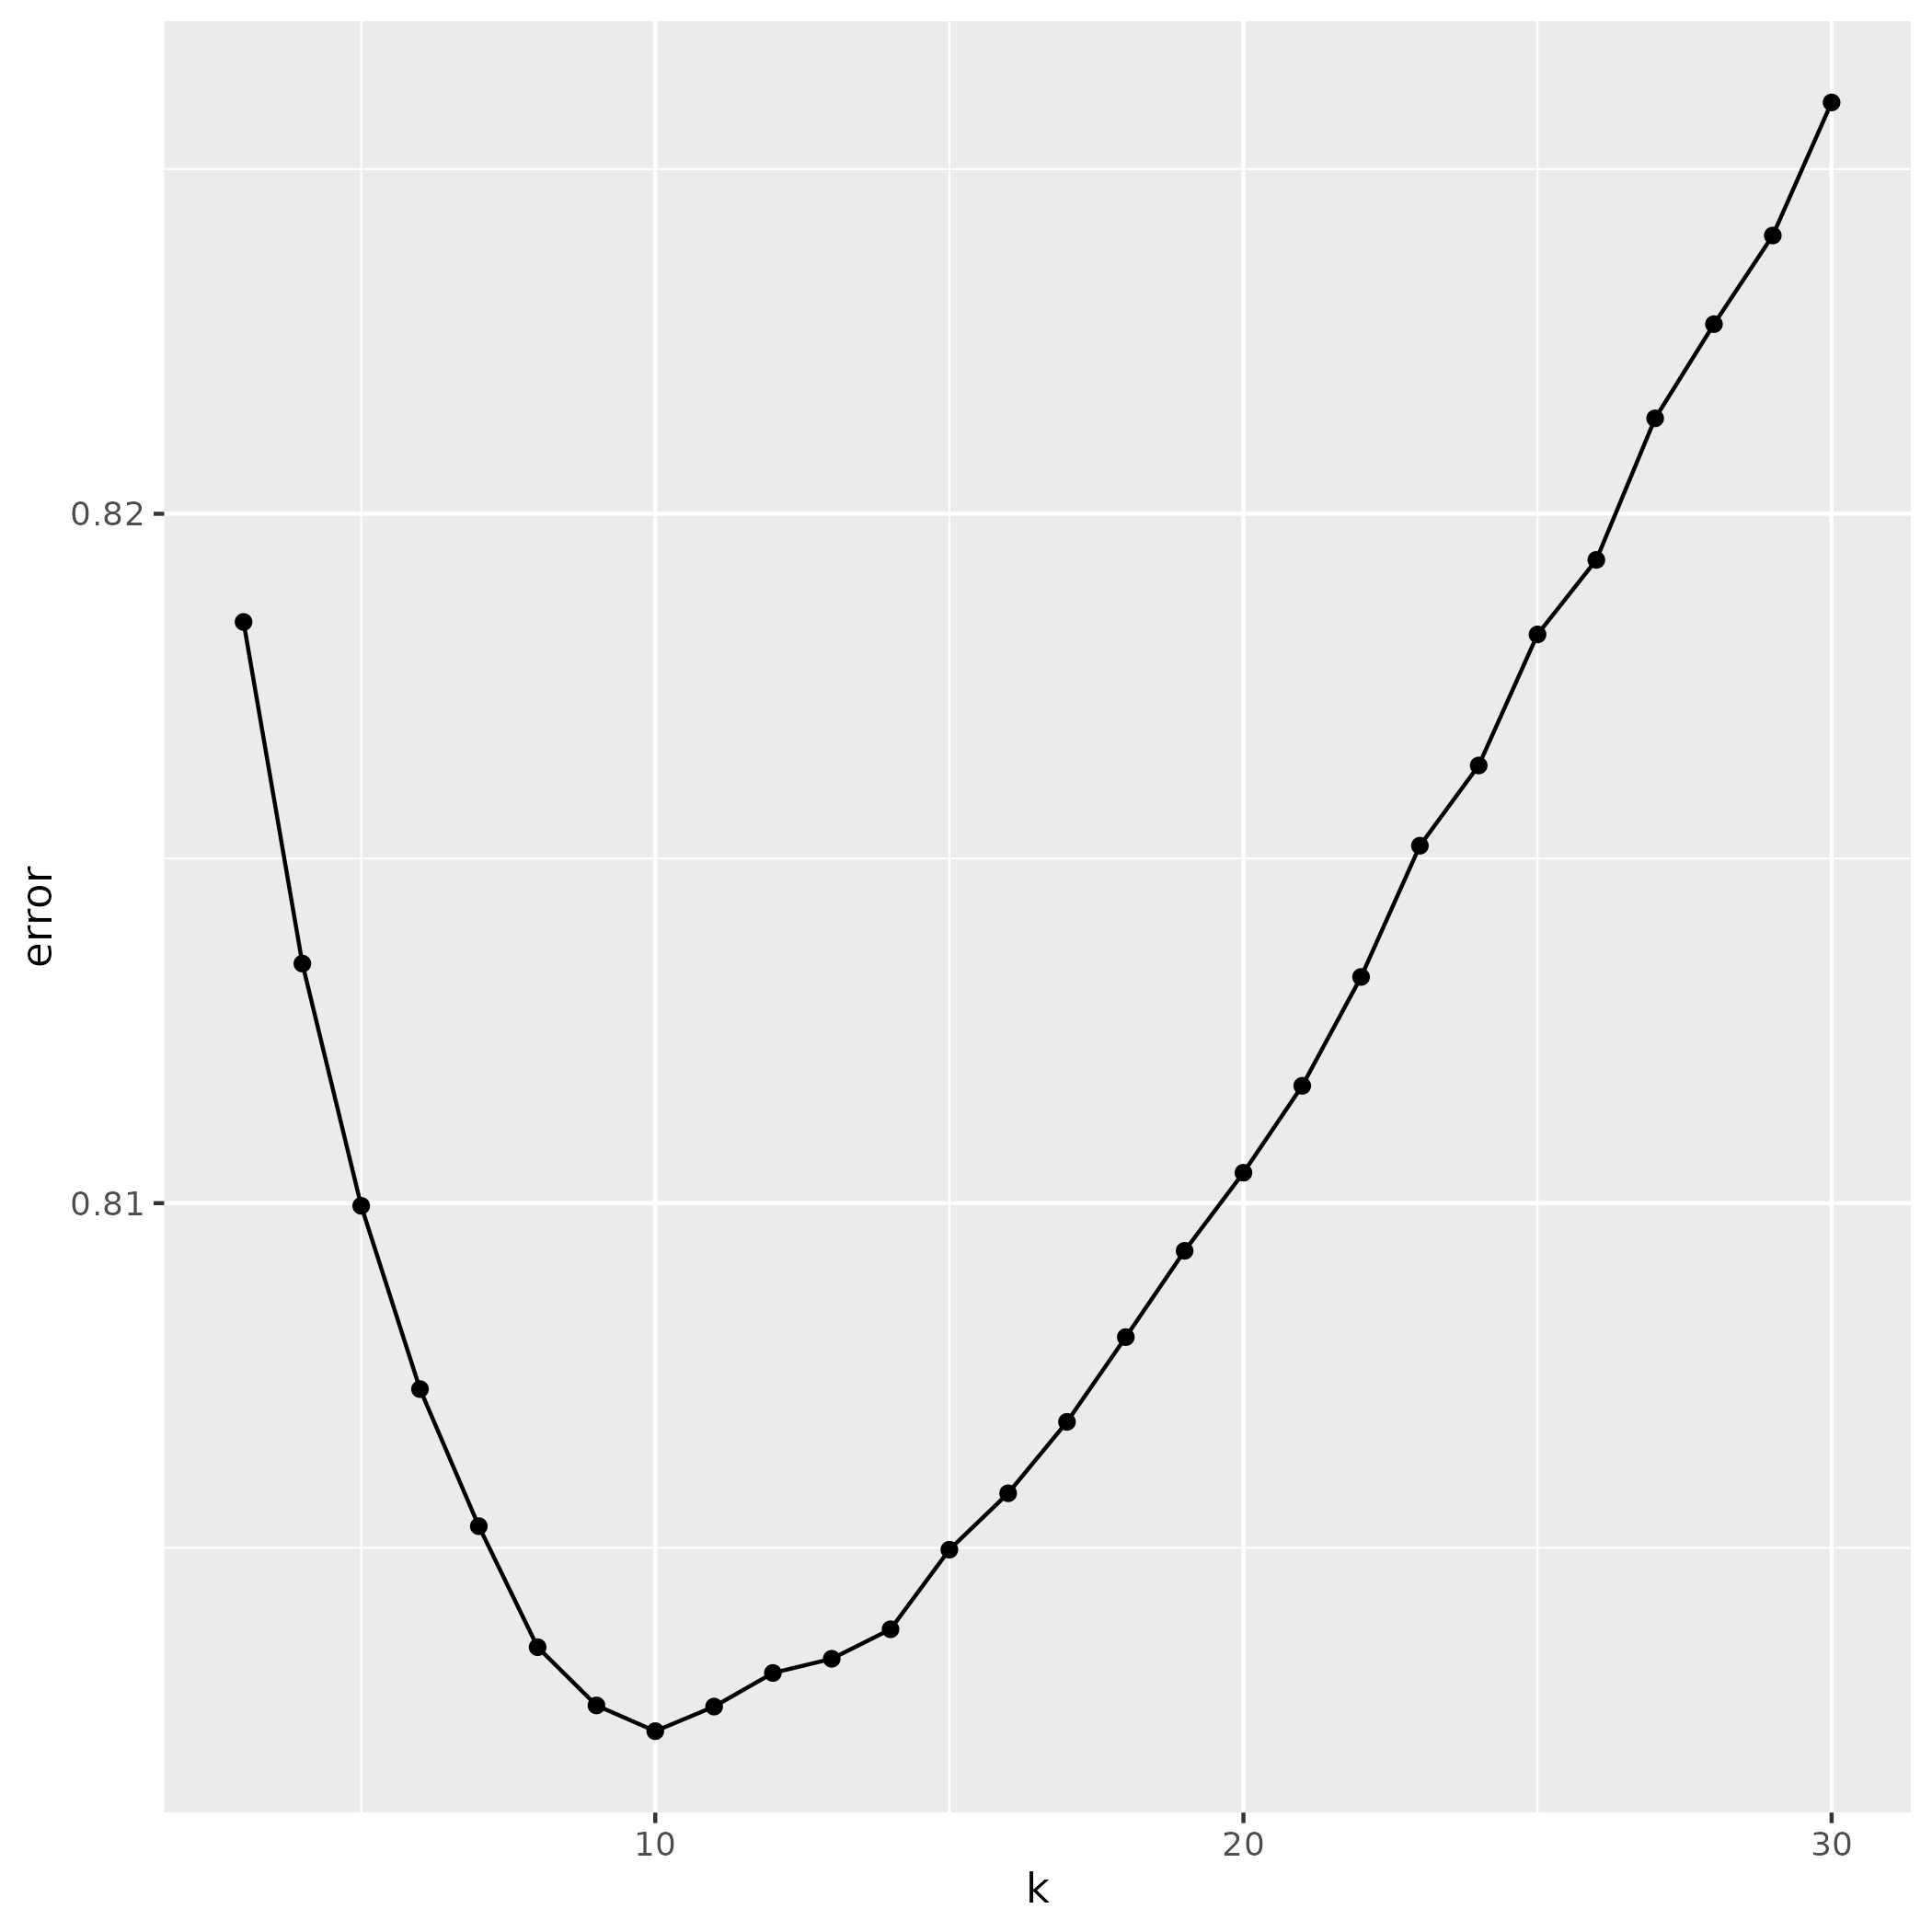
\includegraphics{./model-bias-no-movies.png}
\caption{With bias but without movies data}
\end{figure}

\begin{figure}
\centering
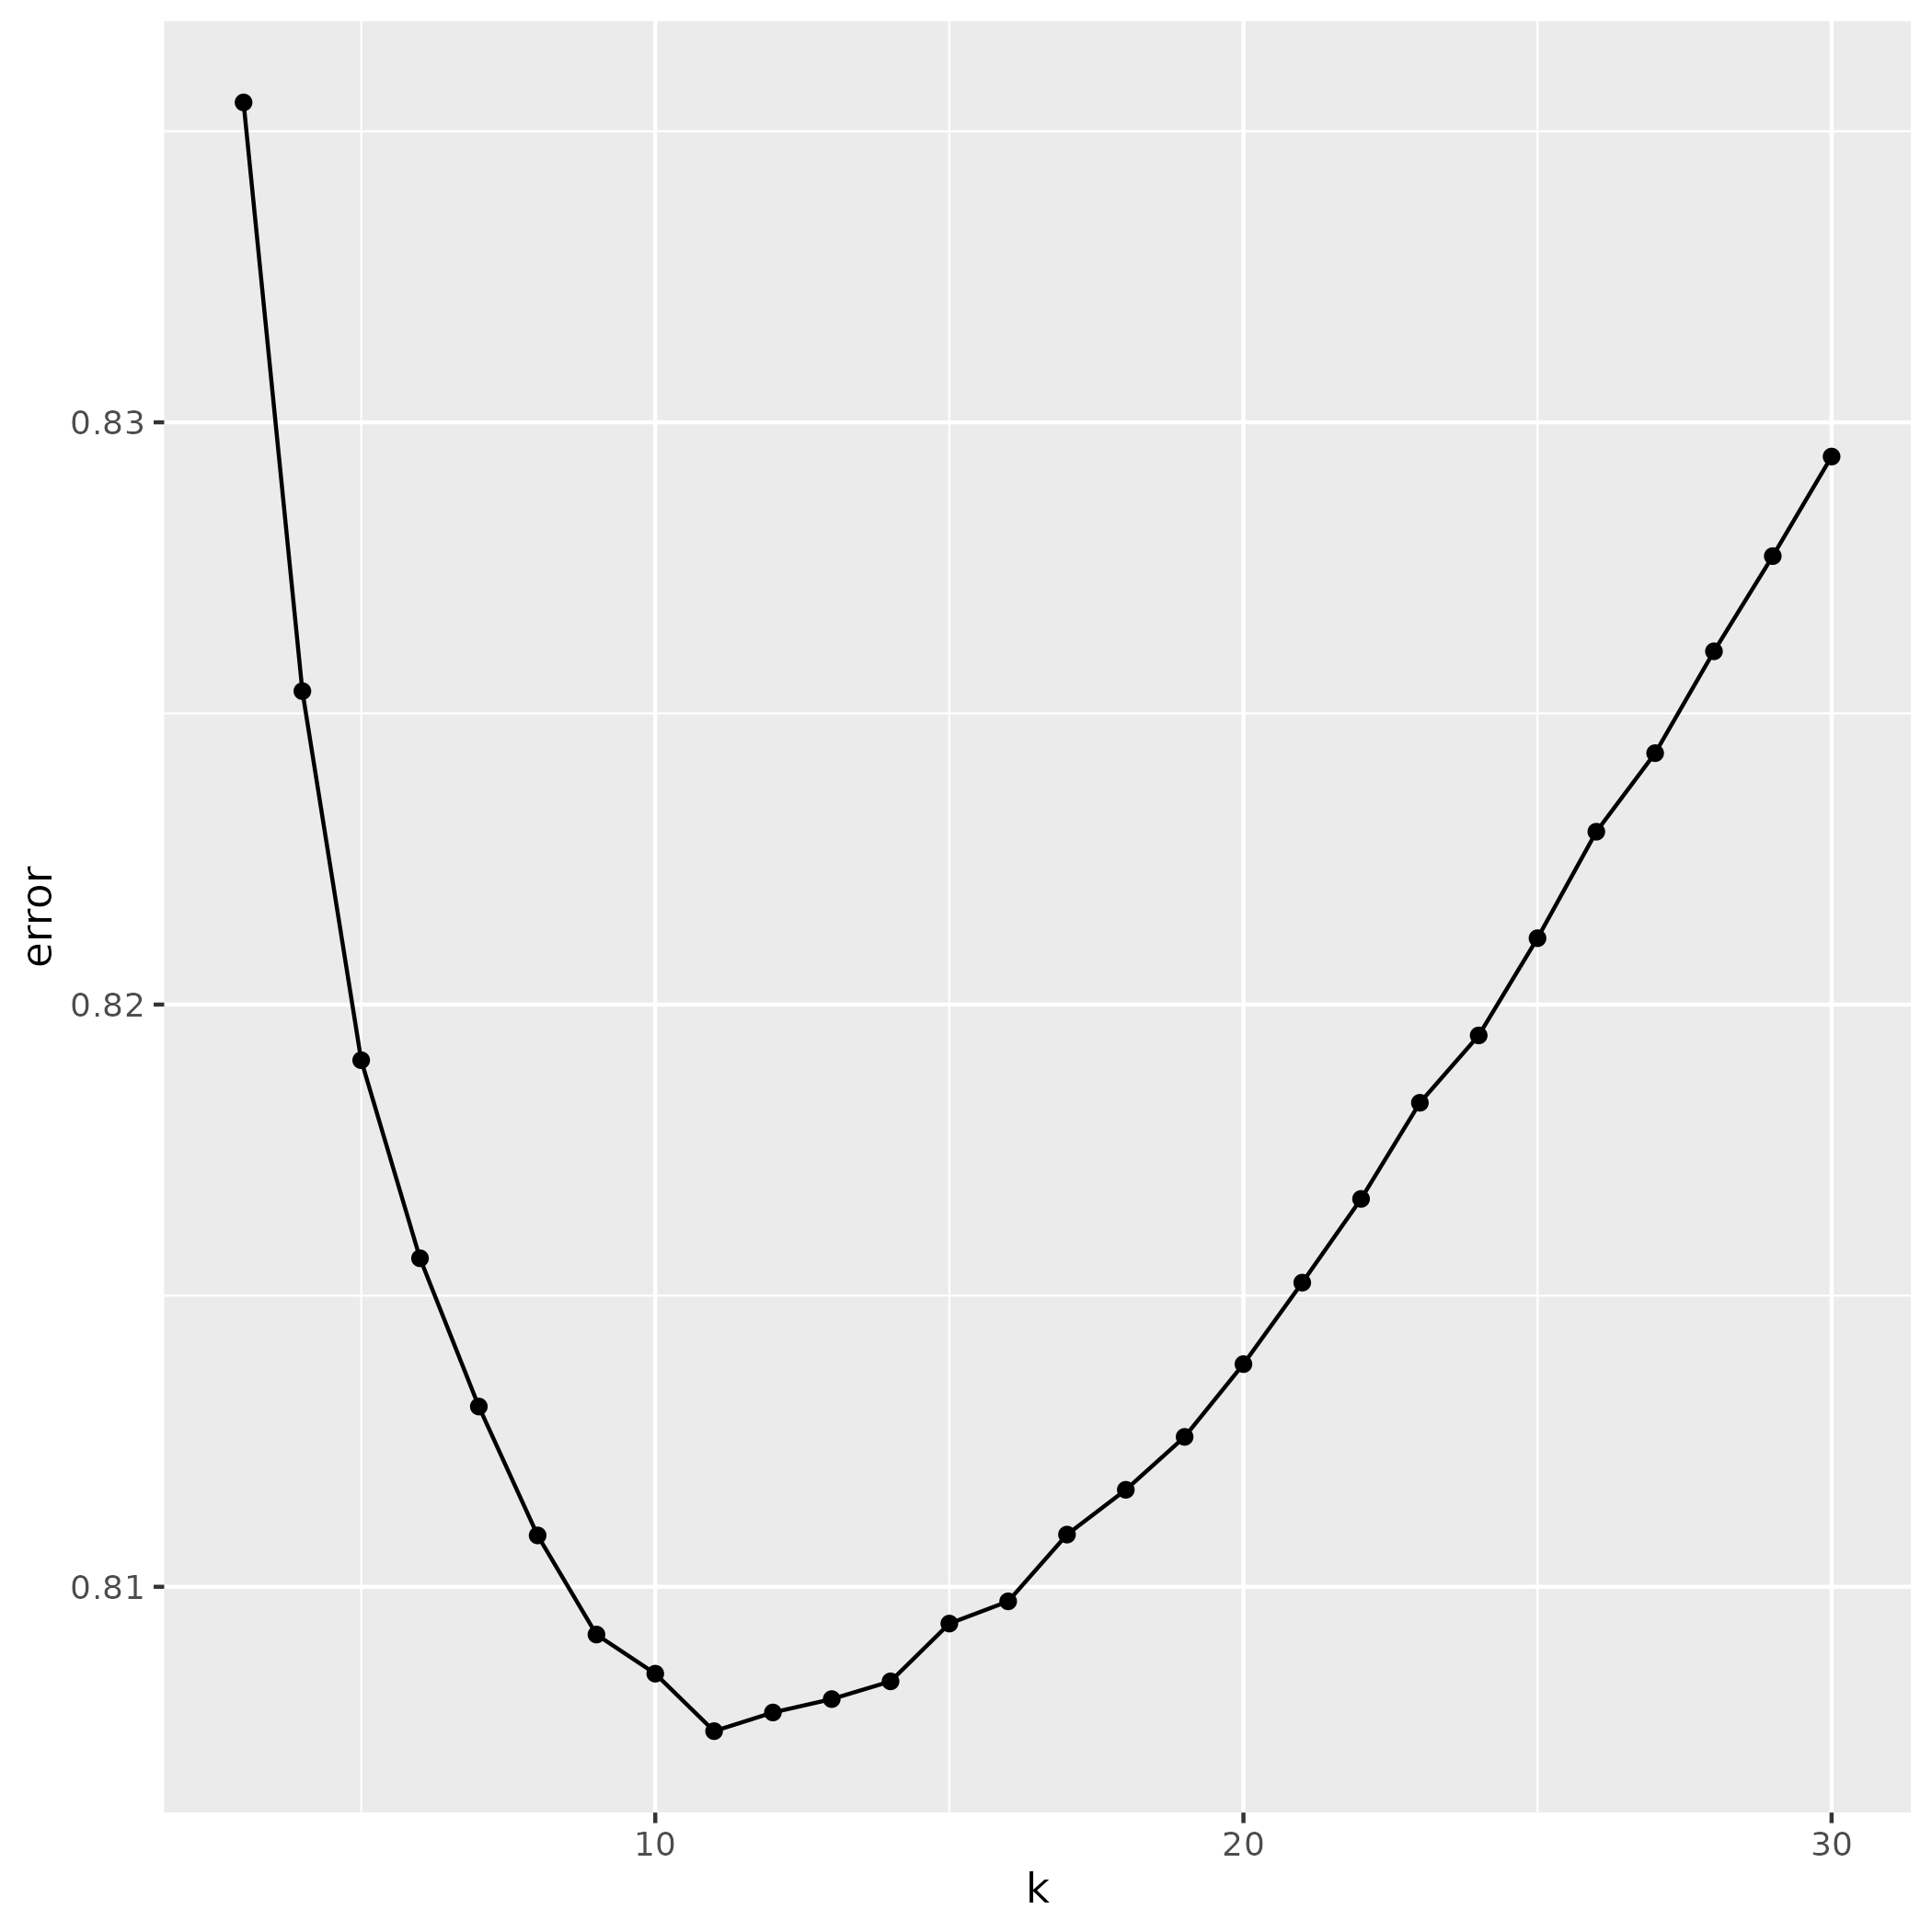
\includegraphics{./model-no-bias-with-movies.png}
\caption{Without bias but with movies data}
\end{figure}

\begin{figure}
\centering
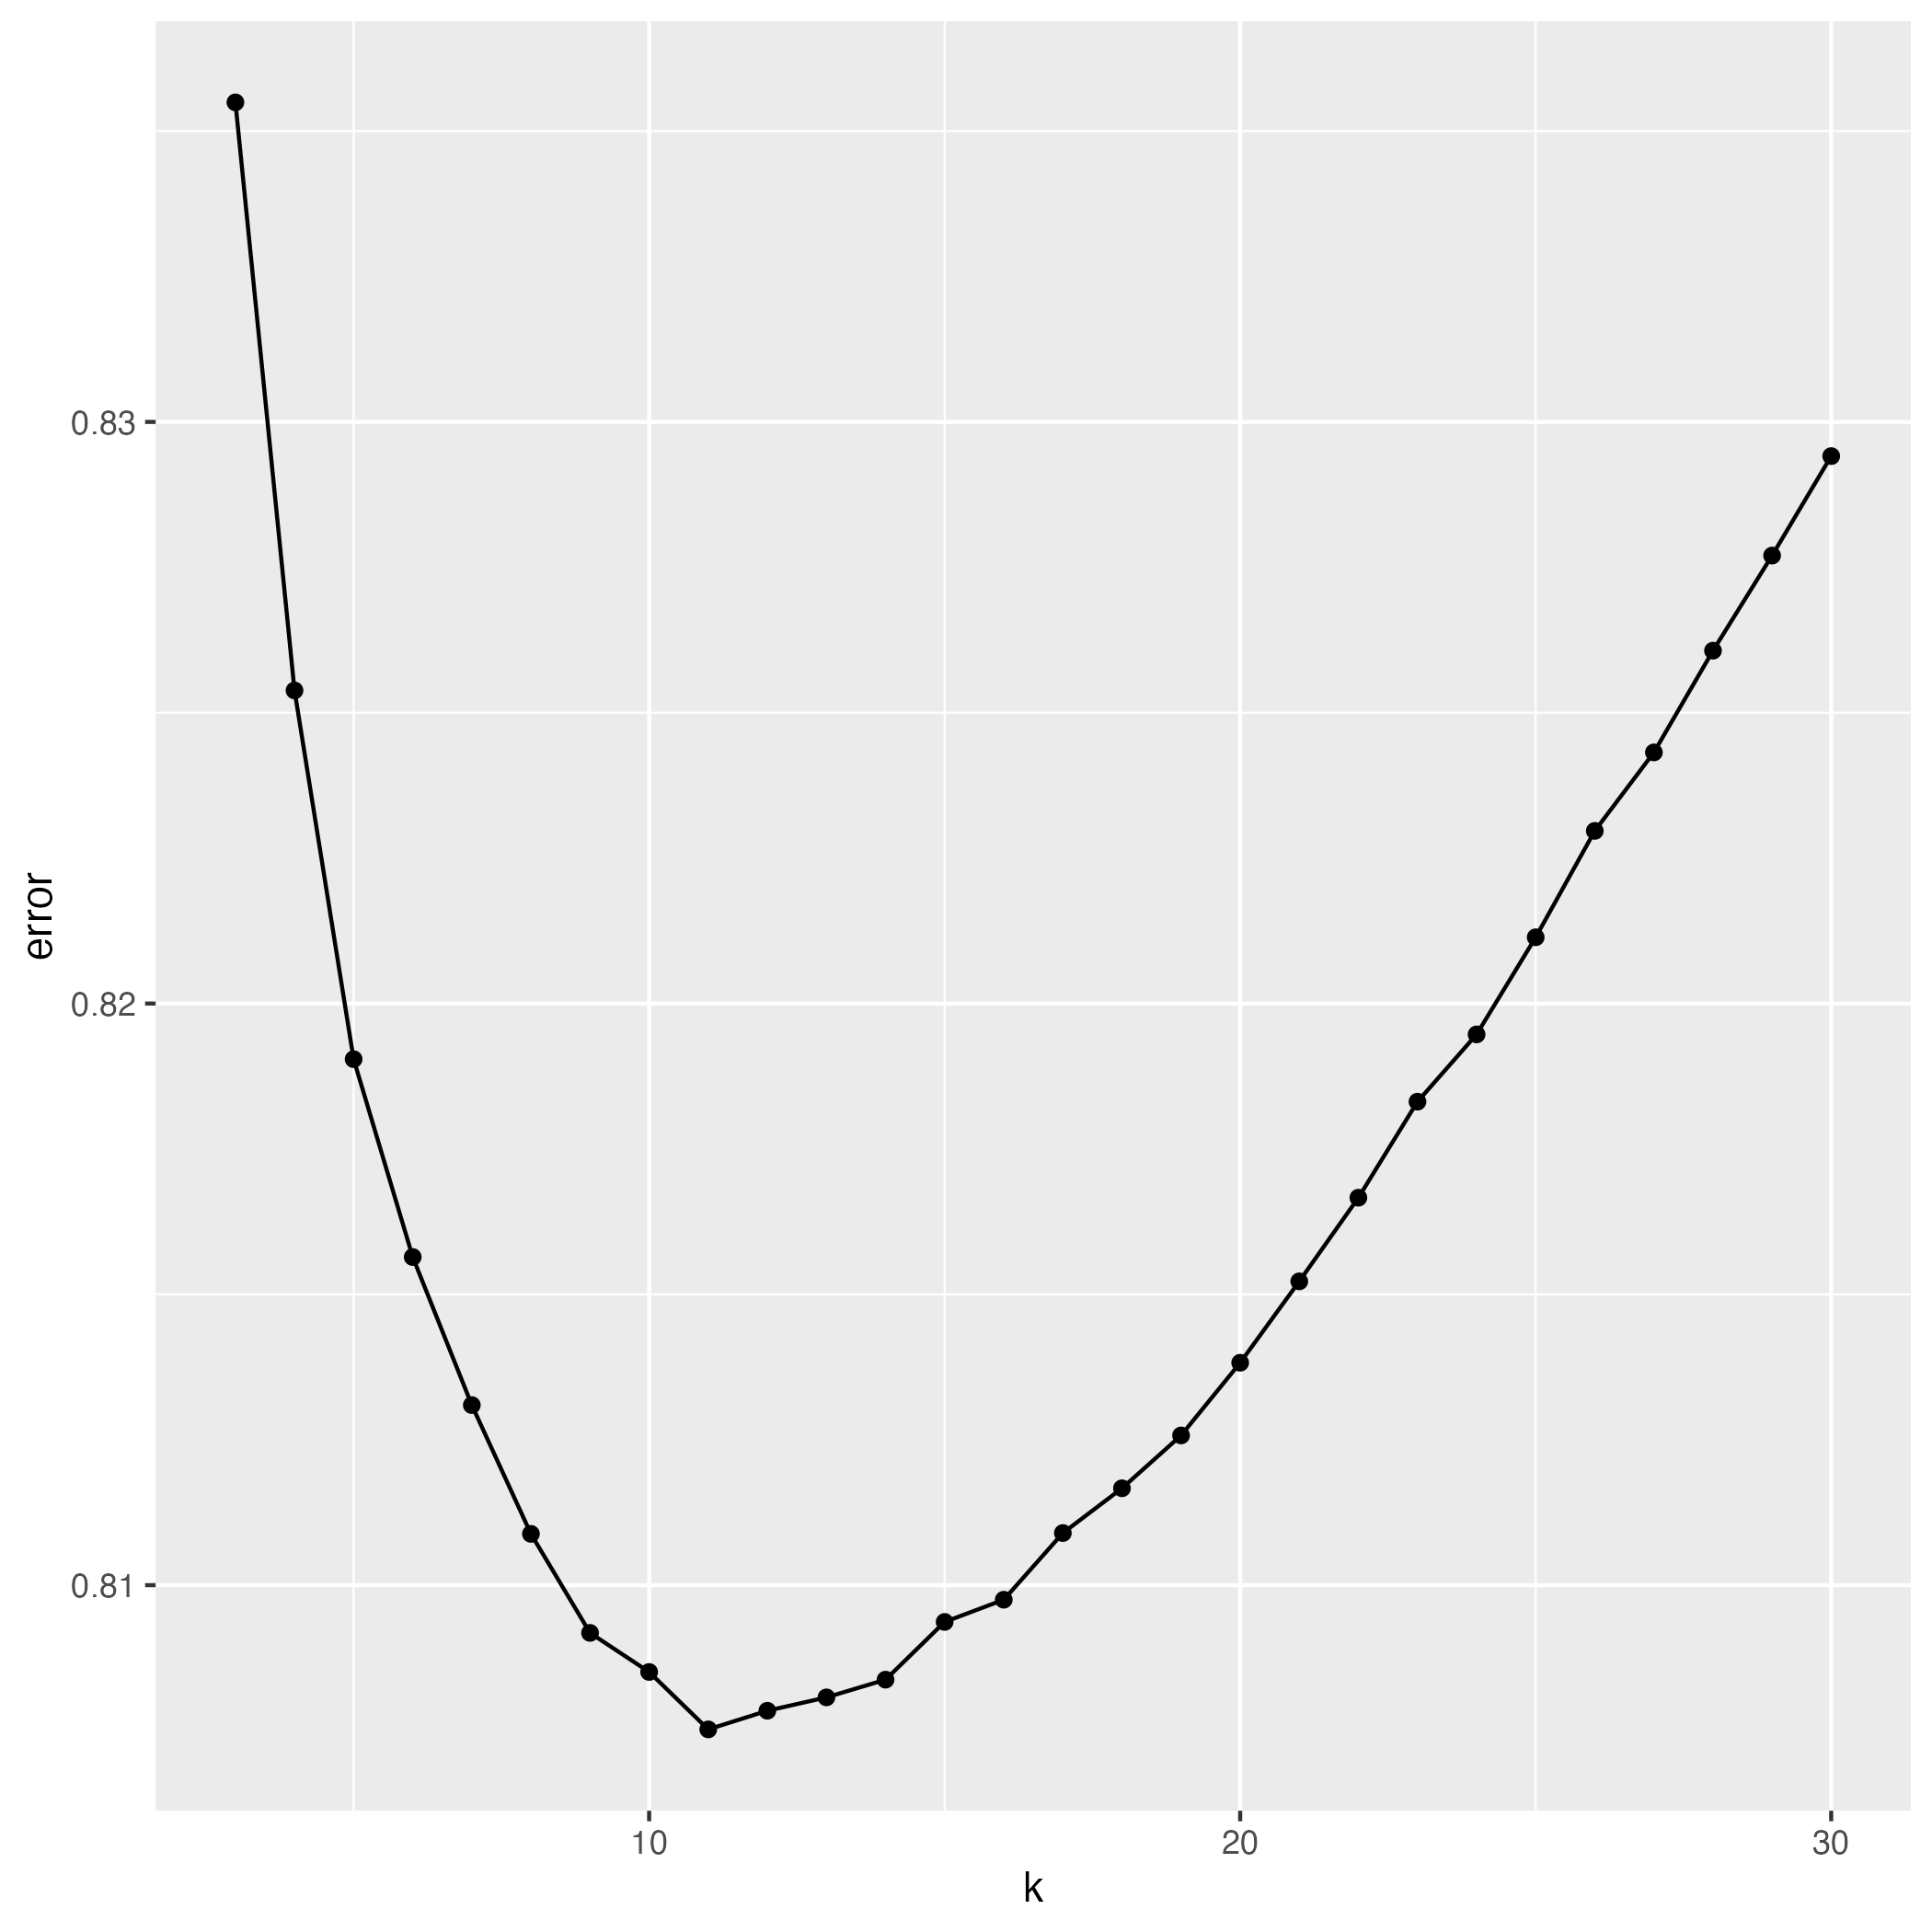
\includegraphics{./model-no-bias-no-movies.png}
\caption{Without bias and movies data}
\end{figure}

The three last chart show us the Bias-Variance tradeoff. We can clearly
observe that at a certain times, after decreasing the RMSE start
increasing, meaning that the variance has increased more than the bias,
leading us into an overfitting situation. The value of K where the RMSE
is the lowest is the best model.

The first graph is different than the 3 last ones because it has
decreased during many steps before being stable. We can ask ourselves
that maybe it can improve with larger value of \(k\).

After plotting the model, we found the best \(K\). The following table
resume the results

\begin{longtable}[]{@{}rcl@{}}
\toprule\noalign{}
Models & Best K & RMSE \\
\midrule\noalign{}
\endhead
\bottomrule\noalign{}
\endlastfoot
Model-ByFy & 29 & 0.831525473100835 \\
Model-ByFn & 10 & 0.802341082970225 \\
Model-BnFy & 11 & 0.807520656630341 \\
Model-BnFn & 11 & 0.807520656630341 \\
\end{longtable}

After this process, from the result in the table above, we can notice
that the model with the minimal RMSE on validation set is the model
\texttt{Model-ByFn} that the one \textbf{with bias but without movie
data}.

We then train the whole data, that is the \texttt{edx} data with that
parameters.

\begin{Shaded}
\begin{Highlighting}[]
\NormalTok{model }\OtherTok{\textless{}{-}} \FunctionTok{CMF}\NormalTok{(X, }\AttributeTok{k =}\NormalTok{ k.min, }\AttributeTok{method =} \StringTok{\textquotesingle{}lbfgs\textquotesingle{}}\NormalTok{,}
            \AttributeTok{user\_bias =} \ConstantTok{TRUE}\NormalTok{, }\AttributeTok{item\_bias =} \ConstantTok{TRUE}\NormalTok{,}
            \AttributeTok{center =} \ConstantTok{TRUE}\NormalTok{,}
            \CommentTok{\# NA\_as\_zero = TRUE, }
            \AttributeTok{nthreads =} \DecValTok{1}\NormalTok{, }\AttributeTok{verbose =} \ConstantTok{FALSE}\NormalTok{, }\AttributeTok{seed =} \DecValTok{1}\NormalTok{)}
\end{Highlighting}
\end{Shaded}

The model obtain is then use to predict the rating on the
\texttt{final\_holdout\_test} data set.

\begin{Shaded}
\begin{Highlighting}[]
\NormalTok{predictions }\OtherTok{\textless{}{-}} \FunctionTok{predict}\NormalTok{(model, }\AttributeTok{user=}\NormalTok{X.fht}\SpecialCharTok{$}\NormalTok{userId, }\AttributeTok{item=}\NormalTok{X.fht}\SpecialCharTok{$}\NormalTok{movieId)}
\NormalTok{fht\_error }\OtherTok{\textless{}{-}} \FunctionTok{RMSE}\NormalTok{(X.fht}\SpecialCharTok{$}\NormalTok{rating, predictions)}
\NormalTok{fht\_error}
\end{Highlighting}
\end{Shaded}

We obtain the \texttt{RMSE} equal to \textbf{0.794544360572509}

\section{Conclusion}\label{conclusion}

We were asked to build a model for predicting rating from user on a
movie. After some research, we heard that it's a machine learning
problem called recommendation system. Multiple approaches exist and we
decided to work on a hybrid approach consisting of mixing collaborative
filtering and content-based filtering. We then propose the find the best
models between 4 defined models. We found the best one after tuning each
of them. We finally get the best model that gave us a RMSE of
\textbf{0.794544360572509} of the hold-out set.

Next, we are going to compare the 4 models using a cross-validation
approach where the different folds will be created like this

\begin{Shaded}
\begin{Highlighting}[]
\NormalTok{X.folds }\OtherTok{\textless{}{-}} \FunctionTok{createFolds}\NormalTok{(}\AttributeTok{y =}\NormalTok{ X}\SpecialCharTok{$}\NormalTok{rating, }\AttributeTok{k =}\NormalTok{ MAX\_FOLDS, }\AttributeTok{list =} \ConstantTok{TRUE}\NormalTok{, }\AttributeTok{returnTrain =} \ConstantTok{TRUE}\NormalTok{)}

\NormalTok{X.fold.train }\OtherTok{=} \FunctionTok{list}\NormalTok{()}
\NormalTok{X.fold.test }\OtherTok{=} \FunctionTok{list}\NormalTok{()}
\NormalTok{X.fold.movies }\OtherTok{=} \FunctionTok{list}\NormalTok{()}

\ControlFlowTok{for}\NormalTok{ (f }\ControlFlowTok{in} \DecValTok{1}\SpecialCharTok{:}\NormalTok{MAX\_FOLDS) \{}
\NormalTok{  fold }\OtherTok{\textless{}{-}}\NormalTok{ X.folds[[f]]}
  
\NormalTok{  fold.train }\OtherTok{\textless{}{-}}\NormalTok{ X[fold, ]}
\NormalTok{  fold.movies }\OtherTok{\textless{}{-}}\NormalTok{ X.movies[fold, ]}
  
\NormalTok{  temp }\OtherTok{\textless{}{-}}\NormalTok{ X[}\SpecialCharTok{{-}}\NormalTok{fold, ]}
  
  \CommentTok{\# Make sure userId and movieId in test set are also in train set}
\NormalTok{  fold.test }\OtherTok{\textless{}{-}}\NormalTok{ temp }\SpecialCharTok{\%\textgreater{}\%} 
    \FunctionTok{semi\_join}\NormalTok{(fold.train, }\AttributeTok{by =} \StringTok{"movieId"}\NormalTok{) }\SpecialCharTok{\%\textgreater{}\%}
    \FunctionTok{semi\_join}\NormalTok{(fold.train, }\AttributeTok{by =} \StringTok{"userId"}\NormalTok{)}
  
  \CommentTok{\# Add rows removed from final hold{-}out test set back into edx set}
\NormalTok{  removed }\OtherTok{\textless{}{-}} \FunctionTok{anti\_join}\NormalTok{(temp, fold.test)}
\NormalTok{  fold.train }\OtherTok{\textless{}{-}} \FunctionTok{rbind}\NormalTok{(fold.train, removed)}
  
\NormalTok{  X.fold.train[[f]] }\OtherTok{\textless{}{-}}\NormalTok{ fold.train}
\NormalTok{  X.fold.test[[f]] }\OtherTok{\textless{}{-}}\NormalTok{ fold.test}
\NormalTok{  X.fold.movies[[f]] }\OtherTok{\textless{}{-}}\NormalTok{ fold.movies}
\NormalTok{\}}
\end{Highlighting}
\end{Shaded}

A cross-validation approach, will be used to compare the 4 models
instead of training/validation data sets approach.

\end{document}
